\chapter{Конструкторская часть}

В данном разделе будут представлены схемы алгоритмов сортировки выбором, Шеллом и гномьей сортировки и вычислены трудоемкости указанных алгоритмов.

\section{Разработка алгоритмов}

На рисунках представлены схемы алгоритмов сортировки выбором, Шеллом и гномьей сортировки.

\begin{figure}[H]
	\begin{center}
		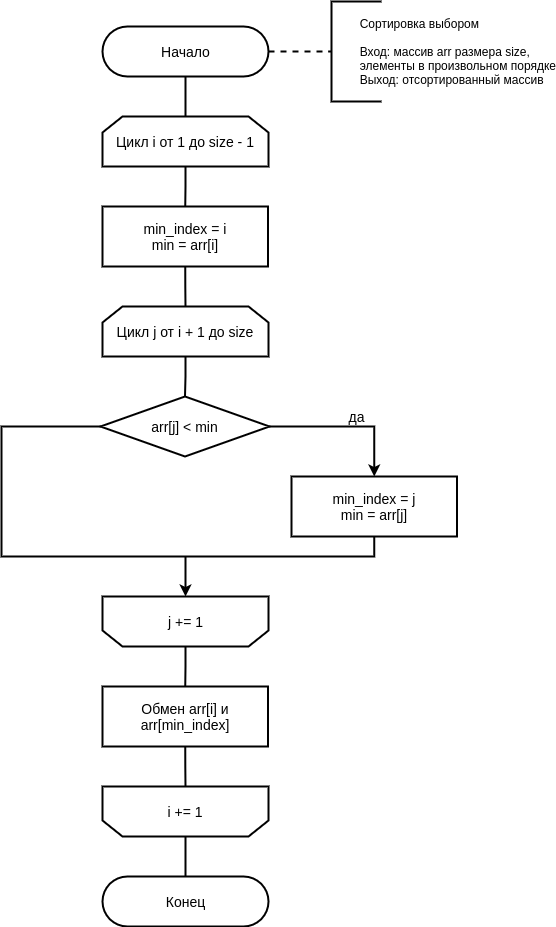
\includegraphics[scale=0.4]{img/selection_sort.png}
	\end{center}
	\captionsetup{justification=centering}
	\caption{Схема алгоритма сортировки выбором}
	\label{img:selection_sort}
\end{figure}

\begin{figure}[H]
	\begin{center}
		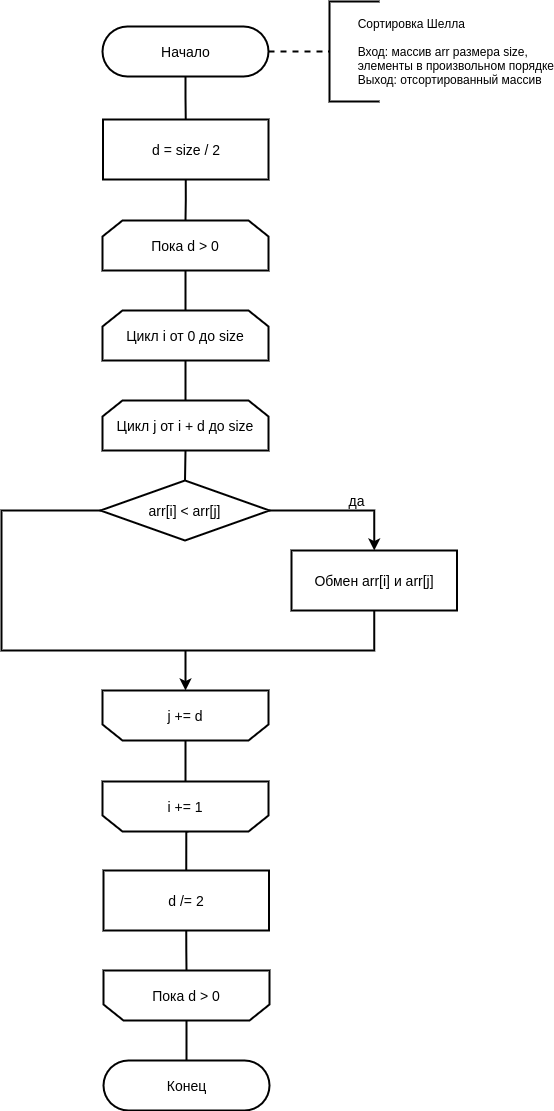
\includegraphics[scale=0.5]{img/shell_sort.png}
	\end{center}
	\captionsetup{justification=centering}
	\caption{Схема алгоритма сортировки Шелла}
	\label{img:shell_sort}
\end{figure}

\newpage

\begin{figure}[H]
	\begin{center}
		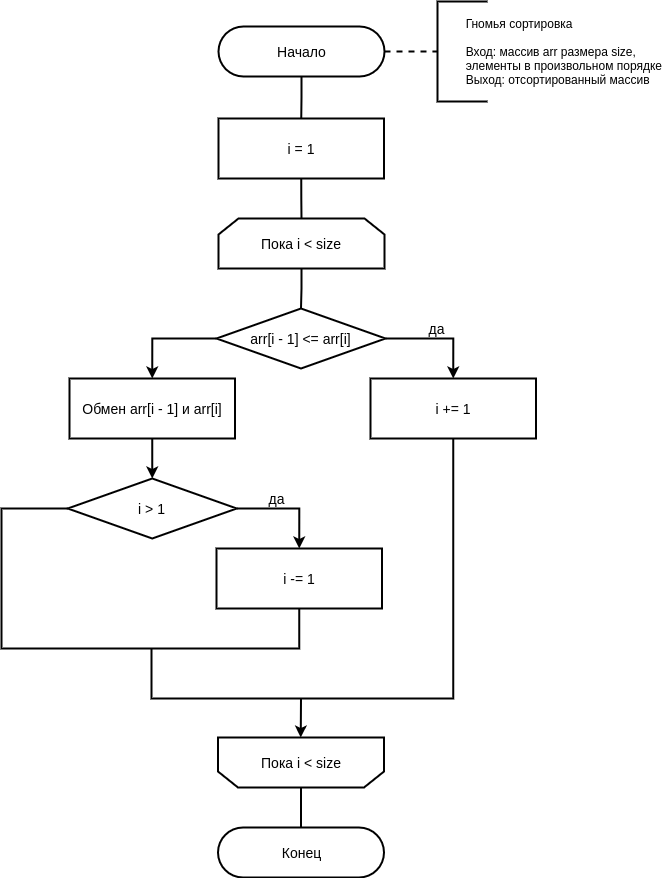
\includegraphics[scale=0.5]{img/gnome_sort.png}
	\end{center}
	\captionsetup{justification=centering}
	\caption{Схема алгоритма гномьей сортировки}
	\label{img:gnome_sort}
\end{figure}

\section{Модель вычислений для оценки трудоёмкости алгоритмов}

Для определения трудоемкости алгоритмов необходимо ввести модель вычислений:

\begin{enumerate}
	\item операции из списка (\ref{for:operations}) имеют трудоемкость равную 1;
	\begin{equation}
		\label{for:operations}
		+, -, /, *, \%, =, +=, -=, *=, /=, \%=, ==, !=, <, >, <=, >=, [], ++, {-}-
	\end{equation}
	\item трудоемкость оператора выбора \code{if условие then A else B} рассчитывается, как (\ref{for:if});
	\begin{equation}
		\label{for:if}
		f_{if} = f_{\text{условия}} +
		\begin{cases}
			f_A, & \text{если условие выполняется,}\\
			f_B, & \text{иначе.}
		\end{cases}
	\end{equation}
	\item трудоемкость цикла рассчитывается, как (\ref{for:cycle});
	\begin{equation}
		\label{for:cycle}
		f_{for} = f_{\text{инициализации}} + f_{\text{сравнения}} + N(f_{\text{тела}} + f_{\text{инкремент}} + f_{\text{сравнения}})
	\end{equation}
	\item трудоемкость вызова функции равна 0.
\end{enumerate}

\section{Трудоёмкость алгоритмов}

\subsection{Алгоритм сортировки выбором}

\subsection{Алгоритм гномьей сортировки}

Трудоемкость в лучшем случае (\ref{for:gnome_best}):

\begin{equation}
	\label{for:gnome_best}
    f_{best} = 1 + N(4 + 1) = 5N + 1 = O(N)
	% f_{best} = -3 + \frac{3}{2} N + \approx \frac{3}{2} N = O(N)
\end{equation}

Трудоёмкость в худшем случае (\ref{for:gnome_worst}):
\begin{equation}
	\label{for:gnome_worst}
    f_{worst} = 1 + N(4 + (N - 1) * (7 + 1 + 2)) = 10N^2 - 6N + 1 = O(N^2)
	% f_{worst} = -3 - 8N + 8N^2 \approx 8N^2 = O(N^2)
\end{equation}

\subsection{Алгоритм сортировки Шелла}

Трудоемкость данного алгоритма может быть рассчитана с использова-
нием той же модели подсчета трудоемкости.

Трудоемкость алгоритма сортировки Шелла:

\begin{itemize}
	\item в лучшем случае - $O(N^2)$;
	\item в худшем случае - $O(Nlog^2N)$.
\end{itemize}

\section*{Вывод}

Были представлены схемы алгоритмов сортировки выбором, Шеллом и гномьей сортировки. Был проведен сравнительный анализ трудоемкостей указанных алгоритмов.
